
%%%%%%%%%%%%%%%%%%%%%%%%%%%%%%%%%%%%%%%%%%%%%%%%%%%%%%%%%%%%%%%%%%%%%%%%%%%
%%% NEUTRONICS

\begin{frame}{Equations for the model - Neutronics}

  \tiny

  \begin{columns}[T]
  \begin{column}{7cm}

    For the neutron field we use:

    \begin{block}{1D two-group neutron diffusion equations}
      \begin{align}
        \frac{1}{v^{1}} \partial_{t} \Phi^{1} 
        - \partial_{z} \left( D^{1} \partial_{z} \Phi^{1} \right) 
        + \Sigma_{r}^{1} \Phi^{1}
        - \frac{1}{\lambda} \nu \Sigma_{f}^{1} \Phi^{1}
        - \frac{1}{\lambda} \nu \Sigma_{f}^{2} \Phi^{2}
        & = 0 \nonumber \\
        \frac{1}{v^{2}} \partial_{t} \Phi^{2} 
        - \partial_{z} \left( D^{2} \partial_{z} \Phi^{2} \right) 
        + \Sigma_{r}^{2} \Phi^{2}
        - \Sigma_{s}^{1 \rightarrow 2} \Phi^{1}
        & = 0 \nonumber
      \end{align}
    \end{block}

    Neutron flux in group $ g $: $ \Phi^{g} = \Phi^{g}(t,z) $
    
    We denote "1" the fast and "2" the thermal groups.

    \begin{block}{Vacuum boundary conditions}
      \begin{align}
        \Phi^{g} = 0 
        \quad \mbox{at } z = 0, Z \nonumber
      \end{align}
    \end{block}

  \end{column}

  \begin{column}{5cm}

    Model assumptions:
    \begin{itemize}
    \item no dependence of the neutron field on the $ r $ coordinate $ \Rightarrow $ $ \nabla \cdot D^{g} \nabla \rightarrow \partial_{z} D^{g} \partial_{z} $
    \item only two energy groups: $ g = 1, 2 $
    \item all fission neutrons will be born in the fast group: $ \chi^{1} = 1 $ and $ \chi^{2} = 0 $
    \item no upscattering: $ \Sigma_{s}^{2\rightarrow 1} = 0 $
    \end{itemize}
 
    \vspace{.5cm}

    The cross sections and the diffusion coefficients are functions of the moderator density $ \rho_{m} $ and the temperature $ T_{eff} $ defined as:
    \begin{align}
      T_{eff} = 
      \alpha \left. T(t,z,r) \right|_{r=0} 
      + (1-\alpha) \left. T(t,z,r) \right|_{r=R_{fuel}} \nonumber
    \end{align}
    (A closure relation gives $ \rho_{m} $ as a function of the enthalpy $ H $ and the pression $ P $)

  \end{column}
  \end{columns}

\end{frame}


%%%%%%%%%%%%%%%%%%%%%%%%%%%%%%%%%%%%%%%%%%%%%%%%%%%%%%%%%%%%%%%%%%%%%%%%%%%
%%% HEAT TRANSFER

\begin{frame}{Equations for the model - Fuel pin heat transfer}

  \tiny

  \begin{columns}
  \begin{column}{8cm}

    For the fuel pin heat transfer, we consider:

    \begin{block}{Heat conduction equations through fuel pin and cladding}
      \begin{align}
        \rho_{fuel} C_{p}^{fuel} \partial_{t} T^{fuel} 
        - (1/r) \partial_{r} r\ k_{fuel} \partial_{r} T^{fuel} 
        = \sum_{g} \kappa^{g} \Sigma_{f}^{g} \Phi^{g}
        \quad &\mbox{for } 0 < r < R_{fuel} \nonumber \\
        \rho_{clad} C_{p}^{clad} \partial_{t} T^{clad} 
        - (1/r) \partial_{r} r\ k_{clad} \partial_{r} T^{clad} 
        = 0 \quad &\mbox{for } R_{fuel} < r < R_{clad} \nonumber
      \end{align}
    \end{block}

    Temperature in the pin fuel and cladding: $ T = T(t,z,r) $ 

%    Thus $ - k \nabla T \rightarrow - k \partial_{r} T $ and
%    $ \nabla \cdot k \nabla \rightarrow (1/r) \partial_{r} r\ k \partial_{r} $.

    \begin{block}{Heat flux from clad to coolant}
      \begin{align}
        -k_{clad} \partial_r T^{clad} = 
        h_{conv} \left( T^{clad} - T_{m} \right)
        \quad &\mbox{at } r = R_{clad} \nonumber
      \end{align}
    \end{block}

      Conductance of the gap between fuel and cladding is taken into account in the model through:
      \begin{align}
        -k_{fuel} \partial_{r} T^{fuel} =
        -k_{clad} \partial_{r} T^{clad} = 
        h_{gap} \left( T^{fuel} - T^{clad} \right)
        \quad &\mbox{at } r = R_{fuel} \nonumber 
      \end{align}

  \end{column}

  \begin{column}{4cm}

    Model assumption:
    \begin{itemize}
    \item no heat conduction along $ z $ axis 
    \item infinitely small gap between fuel and cladding
    \end{itemize}

    \vspace{.5cm}

    Thermal conductivity $ k $, heat capacity $ C_p $, and density $ \rho $, depend on the temperature itself $ \Rightarrow $ nonlinearity

    \vspace{.5cm}

%    In the source term, $ \kappa^{g} $ is the energy released per fission.

  \end{column}
  \end{columns}

\end{frame}


%%%%%%%%%%%%%%%%%%%%%%%%%%%%%%%%%%%%%%%%%%%%%%%%%%%%%%%%%%%%%%%%%%%%%%%%%%%
%%% FLUID DYNAMICS

\begin{frame}{Equations for the model - Fluid flow}

  \tiny

  \begin{columns}
  \begin{column}{8cm}

    For the coolant we use:

    \begin{block}{Enthalpy balance}
      \begin{align}
        \left[ \partial_{t} \rho_{m} 
        + \rho_{m} v \partial_{z} \right] H\ S_{h}
        = - k^{clad} \partial_{r} T (R_{clad}) \Delta z\ 2 \pi R_{clad} \nonumber
      \end{align}
    \end{block}

    Enthalpy of the coolant per unit mass: $ H = H(t,z) $

    \begin{block}{Inlet enthalpy}
      \begin{align}
        H = H_{in} \quad \mbox{at } z = 0 \nonumber
      \end{align}
    \end{block}

  Heat flux from the fuel pin: $ - k^{clad} \partial_{r} T (R_{clad}) = h_{conv} \left( T (R_{clad}) - T_{m} \right) $
  \end{column}

  \begin{column}{4cm}

    Model assumptions:
    \begin{itemize}
    \item pression $ P $ is fixed (155 bars)
    \item fluid flows along $z$-axis
    \item constant mass flow rate $ (\rho_{m} v) S_{h} $
    \end{itemize}

    \vspace{.5cm}

    There is a one-to-one relationship between $ \rho_{m} $, $ T_{m} $ and $ H $

  \end{column}
  \end{columns}

\end{frame}


%%%%%%%%%%%%%%%%%%%%%%%%%%%%%%%%%%%%%%%%%%%%%%%%%%%%%%%%%%%%%%%%%%%%%%%%%%%
%%% SOLVER

\begin{frame}{Newton's method equation solver}

  \tiny

  \begin{columns}
  \begin{column}{9cm}
    Let $ \bs{u} = \bv \Phi\\ T\\  H\\ \ev $ be the vector of unknown coefficients.

  \begin{block}{Newton's method}
    We put the nonlinear problem under the form:
    $
      \bs{r} ( \bs{u} ) = 0 \nonumber
    $,
    where $ \bs{r} $ is a nonlinear residual vector that we want to minimize.

    We take an initial ``guess'' $ \bs{u_{0}} $ and we iterate over $ k $ until $ \bs{r} (\bs{u_{k+1}} ) $ is sufficiently close to the zero vector:
    \begin{align}
      \bs{u}_{k+1} = \bs{u}_{k} 
      - \bs{J}^{-1}(\bs{u}_{k}) \bs{r}(\bs{u}_{k}) \nonumber
    \end{align}
    Here the $ J^{-1} $ is the inverse of the jacobian matrix

    $ J (\bs{u}) = D\bs{r} / D\bs{u} $ (= matrix of all 1st-order partial derivatives of the residual $ \bs{r} $ with respect to the vector of unknown $ \bs{u} $)

  \end{block}

    Remark: Newton's method will converge in one iteration for a linear problem.

  \end{column}
  \begin{column}{3cm}

    \hspace{.5cm}
    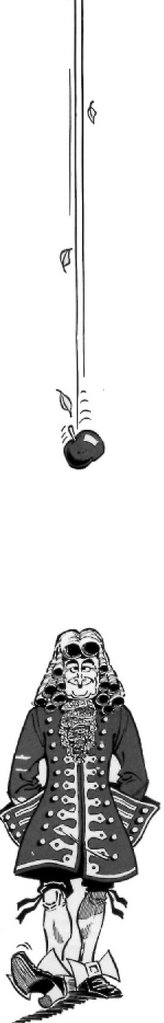
\includegraphics[width=1cm]{figures/newton}

  \end{column}
  \end{columns}

\end{frame}
